

% \begin{figure}[h]
%     \centering
%     \includegraphics[width=5cm, height=4cm]{Figures/Test_logo.png}
%     \caption{Caption}
%     \label{fig:my_label}
% \end{figure}

\fancyhf{}
\fancyhead[c]{Chapter 4. Timescale Heterogeneiety in Reservoir Computing}% <- added
\fancyfoot[R]{\thepage\ifodd\value{page}\else\hfill\fi}
%\fancyhead[L]{\ifodd\value{page}\relax\else\hfill\fi Ch \thechapter}
%\renewcommand\headrulewidth{0pt}% default ist .4pt
\renewcommand{\plainheadrulewidth}{.4pt}% default is 0pt


\newpage


\section{Abstract}

Biological neural systems exhibit significant heterogeneity in temporal dynamics, with neurons operating 
on a wide range of intrinsic timescales. In contrast, most artificial recurrent networks, including those 
in the reservoir computing (RC) framework, use homogeneous decay parameters across units. In this work, 
we investigate whether introducing decay heterogeneity improves task performance in Echo State Networks (ESNs) and 
Distance-based Delay Networks (DDNs). We evaluate four heterogeneity configurations:homogeneous network, homogeneous 
cluster, heterogeneous network, and heterogeneous cluster, across two benchmark tasks: NARMA-30 and Mackey-Glass. 
Networks are optimized using Covariance Matrix Adaptation Evolution Strategy (CMA-ES), and evaluated on task 
performance, we studied the dynamical stability (Lyapunov exponents), representational dimensionality, and 
linear memory capacity of these networks. Our results show that DDNs consistently outperform ESNs, with 
homogeneous DDNs achieving the highest task performance. Timescale heterogeneity enhances memory 
flexibility in DDNs without compromising stability, while ESNs remain relatively unaffected. These findings 
suggest that structured heterogeneity in intrinsic timescales significantly improves the computational 
capabilities of delay-based recurrent systems.

\newpage


\section {Introduction}

Physical systems such as brains consist of heterogeneous neurons; not just in terms of morphology and molecular composition, but also in their temporal properties \cite{koch1999complexity, habashy2024adapting}. In some cases, temporal differences among neuron types span several orders of magnitude \cite{london2010sensitivity, brunel2003firing, wang2020heterogeneity}. This diversity serves multiple functional roles, including supporting motor control \cite{cavanagh2020diversity}, preserving remote memories \cite{runyan2017distinct}, and enabling spatial memory formation \cite{mcnaughton2006path}. In particular, variation in neuronal time constants and decay dynamics is thought to be critical for temporal processing and memory formation in the brain \cite{hasson2008hierarchical, chu2020long}.

In contrast, artificial neural networks, especially recurrent neural networks and their variants like the reservoir computing (RC) framework, are typically designed with homogeneous units that share identical intrinsic parameters. RC is a powerful approach for modeling temporal sequences \cite{lukovsevivcius2009reservoir}, using high-dimensional dynamical systems such as Echo State Networks (ESNs) \cite{jaeger2001echo}. These networks rely on a fixed, randomly connected recurrent reservoir whose states are linearly combined by a trainable readout layer. This setup simplifies training while maintaining strong performance on memory-intensive and nonlinear tasks. A key hyperparameter in RC systems is the leak or decay rate, which controls how much past information is taken into consideration in each unit, shaping the network's temporal memory \cite{schrauwen2007overview}.

Recently, an extension of ESNs called Distance-based Delay Networks (DDNs) \cite{iacob2022distance} has been introduced. DDNs incorporate non-uniform delays between reservoir units, motivated by the fact that axonal delays are ubiquitous in the brain and that information in physical systems like the brain is constrained by spatial structure and finite signal transmission speed \cite{izhikevich2006polychronization}. Prior work has shown that these delays lead to a redistribution of memory across timescales and can improve task performance compared to standard ESNs \cite{iacob2022distance, soriano2014delay, perez2021neural }.

However, while the role of inter-unit delays has been explored, it remains unclear whether heterogeneity in intrinsic parameters, specifically, decay rates—can further enhance performance in both ESNs and DDNs. Most prior studies assume a single, homogeneous decay parameter across all units, effectively enforcing a single timescale on the reservoir. This may limit the system's ability to capture rich, multi-timescale dynamics, especially in tasks that demand both, short and long-term memory. In contrast, biological neural systems inherently operate with a range of time constants \cite{london2010sensitivity, nam2017diversity, zhou2023temporal}, suggesting that incorporating decay heterogeneity could yield computational benefits.

To investigate this, we design and analyze two sets of reservoir networks, ESNs and DDNs, each implemented in four different configurations. These include a homogeneous setup where all units share a fixed decay value, a fixed-cluster configuration where the reservoir is divided into modules, each with its own fixed decay, a network-heterogeneous configuration where each unit's decay is sampled independently from a common distribution; and a cluster-heterogeneous configuration where different modules sample their decays from different distributions. We evaluate all configurations on two standard benchmark tasks: the NARMA-30 task, which tests nonlinear memory capacity, and the Mackey-Glass task, which involves chaotic time-series prediction. Performance is optimized using Covariance Matrix Adaptation Evolution Strategy (CMA-ES), with task evaluation based on normalized root mean square error (NRMSE) for NARMA and prediction horizon for Mackey-Glass.

Beyond performance, we analyze the networks' internal dynamics to understand the mechanisms underlying any observed differences. We compute Lyapunov exponents to assess dynamical stability and chaotic behavior, measure representational dimensionality using SVD-based metrics, and evaluate linear memory capacity. Our results show that DDNs consistently outperform ESNs across all heterogeneity types, with fixed-cluster DDNs performing best. These findings suggest that structured temporal heterogeneity, particularly when organized in modular clusters, significantly enhances the computational capabilities of reservoir networks for tasks involving memory and temporal dynamics. But the heterogniety requirement is task dependent.  

\newpage


\section{Methods}



\subsection{Network Design}

\subsubsection{Echo State networks }

Echo state networks (ESN) are essentially recurrent networks with fixed weights and randomly connected units given by the following equation: 

\begin{equation}
    x(n+1) = (1-\alpha)x(n) + \alpha f(W_{res}x(n) + b_{res} + W_{in}v(n)) 
\end{equation}

Contrary to RNNS, only the linear readout layer is trained for an ESN in order to optimize it for a task. In the given formulation above, x(n) represents the state of the reservoir at time step n. The size of the reservoir is given by the number of units $N$. $W_{res}$ represents the $N \cdot N$ weight matrix of the reservoir. Symbol $W_{in}$ represents a $N_{in} \cdot N$ input weight matrix. $b_{res}$ represents the bias reservoir weights of size $N$. The symbol $v(n)$ is the input to the reservoir at time step $n$. $\alpha$ is the leak parameter, which decides the importance of previous states on the current state, this acting as memory. This leak parameter can be fixed or distinct for each unit. $f(\cdot)$ is the non-linear activation function, which is usually sigmoid or hyperbolic tangent.     

\subsubsection{Distance based delay networks}

The architecture of Distance based delay networks are similar to ESNs except for the introduction of delays, the delays are implemented by assuming that each unit lies on a 2-D Euclidean space and the distance between two units determine the delay between them. A distance matrix $D$ is computed, where each element $D_{ij}$ represents the distance between units $i$ and $j$ scaled by signal propagation velocity and simulation timestep. A new masked weight matrix $W^{res}_{D=d}$ is created accounting for delays, each element in this matrix is given by the following equation:

\begin{equation}
    W_{i,j,D=d} = \delta_{i,D_{ij}} \cdot W_{i,j} 
\end{equation}

here, d is $\in$ [$1$, $D_{max}$] and $\delta$ is the Kronecker delta operator.  $D_{max}$ is the maximum value delay can take. This method allows for all the weights other than at delay of $d$ to be zero. The final update equation for DDNs is given by: 
\begin{equation}
i(n)  = \sum_{d=0}^{D_{max}} \bigg( W^{res}_{D=d} x(n-d) + W^{in}_{D=d} v(n-d) \bigg ) + b_{res} \\
\end{equation}
\begin{equation}
    x(n) = (1-\alpha) x(n-1) + \alpha f(i(n)) 
\end{equation}

All the parameters in the above set of equations are identical except for the addition of delays. As described in \cite{iacob2022distance}, the delay between individual units are treated as hyperparameters to be optimized. The coordinates are sampled using a Gaussian Mixture model, with $K$ clusters, instead of finding the optimal coordinates for each unit, the GMM model is optimized to find the fitting distribution for each cluster.  

\subsection{Task}

\subsubsection{NARMA-30}
The Nonlinear auto-regressive moving average (NARMA) is a popular benchmark task used to evaluate the performance of RC system. It is a system of equation that is highly non-linear and has clear temporal dependencies, defined by the order parameter. The general system of equation is given by the following equation: 

\begin{equation}
    y(t+1)  = c_1 \cdot y(t)+c_2 \cdot \sum_{i=0}^{p} y(t-i) + c_3 \cdot u(t-p)u(t) +c_4
\end{equation}
Where $c_1$ -- $c_4$ are task parameters, and $p$ is the NARMA order. $y(t)$ is the state of the system at time t, $u(t)$ is the input to the system at time $t$, which is uniformly sampled between $0.0$ and $0.5$.   Essentially the task entails predicting the next state given the serialized previous states, we used the NARMA-30 task to train our networks, the parameters are $p = 29$, $c_1 = 0.2$, $c_2 = 0.004$, $c_3 = 1.5$, and $c_4 = 0.1$. 

\subsubsection{Evaluation}
We evaluated the NARMA-30 task using Normalized root mean squared error (NRMSE) given as follow: 
\begin{equation}
    NRMSE = \frac{1}{\bar{y}}\sqrt{\frac{\sum(y_i - \hat{y}_i)^2}{n}}      
\end{equation}
where $\bar{y}$ is the mean of the ground truth, $y_i$ and $\hat{y}_i$ are ground truth and network readout respectively, $n$ is the total number of elements in the time series.     

\subsubsection{Mackey-Glass}

The discretized Mackey-Glass timeseries is given by the following equation:

\begin{equation}
    x(t+1) = x(t) + \beta\frac{x(t-\tau)}{1+x(t-\tau)^{n}} -\gamma x(t)
\end{equation}
The parameters the following $\tau = 17$, $n = 10$, $\beta = 0.2$ and $\gamma = 0.1$. The aim of this task is to accurately generate the Mackey-Glass sequence as long as possible using the previous step and not receiving any external input or correction. This is done by training the readout layers of the networks for one step ahead prediction.  The performance is measured by a metric called prediction horizon, which measures how many time steps into the future can be predicted by the network accurately within an error margin. The error margins are $\pm 0.1\sigma^{2}_l$, where $\sigma^{2}_l$ is the label variance. 

\subsubsection{Evaluation}
We evaluated the network performance using prediction horizon, which the number of time steps the network can predict the time series within the error margins. 

\subsection{Training}
\subsubsection{CMA-ES Optimization}
The Covariance Matrix Adaptation Evolution Strategy (CMA-ES) \cite{hansen2006the-cma-evoluti} is a widely used evolutionary algorithm for hyperparameter optimization, especially effective for non-convex and high-dimensional problems. CMA-ES consists of a multivariate Gaussian search distribution defined by a mean vector, step-size, and covariance matrix. At each iteration, it samples a population of candidate solutions from this distribution, evaluates their fitness, and updates the mean and covariance matrix to sample future samples from more fitting regions of the search space. The mean vector represents the current best candidate based on the population's progress, while the covariance matrix spans the space of the search distribution. This iterative process enables CMA-ES to efficiently explore complex solution spaces and is robust due to its invariance properties and ability to handle parallel evaluations. In case of ESN and DDN optimization, the mean vectors are the hyperparameters of DDNs and ESNs. Initially, all hyperparameters are roughly made to fall in the same range, after every iteration, a new hyperparameter vector is generated based on the evolution of the multi-variate distribution. Using this new solution vector, networks are generated and are used to perform validation scores. Both ESN and DDN optimizations are run for 200 generations with a population size of 20 for Mackey Glass task and population size 25 for NARMA 30 task. 

\subsubsection{Readout training}
The randomly sampled network is not directly able to perform the task, it is essentially it acts as a temporal kernel that increases the dimensionality of the input and thus increases the linear separability, the activity from a network driven by a random input can be recorded and can be treated as a feature matrix $X$ of size $N\times T$, where $N$ is the number of neurons and $T$ is the number of time steps of the simulation. The output labels $\hat{y}$ and and the corresponding input vector $v(n)$ are ordered vectors of size $T$. The objective function $J$ given by the following equation below is solved using ridge regression trained on network activities: 
\begin{equation}
    J(W_{readout}) = ||XW_{readout}  - \hat{y} ||^2_2 + \lambda || W_{readout}||_2^2
\end{equation}
Optimizing the above equation gives the $W_{readout}$, where $\lambda$ is the regularizing parameter and $W_{readout}$ is the readout. 

\subsection{Lyapunov exponent}

Dynamics of the RC system can be studied by estimating the Lyapunov exponent of the network trajectory, we calculated the Lyapunov exponent of ESNs and DDNs using numerical method, explained by \cite{boedecker2012information}. Lyapunov exponent is given by the following equation: 
\begin{equation}
    \lambda = \lim_{t \to +\infty} ln \bigg ( \frac{\gamma_t}{\gamma_{0}} \bigg )  
    \label{eq:lyapuno}
\end{equation}
The steps involved in the numerical calculation as described by \cite{boedecker2012information} is as follows:
\begin{enumerate}
    \item Two identical networks $X_1$ and $X_2$ were created taking the best sampled networks, a reservoir unit from one of the network $X_1$ was given a small perturbation and the network $X_2$ was kept as is. The initial $L2$ normalized distance between $X_1$ and $X_2$ is therefore $\gamma_0$.   
    \item The network is driven by the input that the respective network is trained on, that is either NARMA-30 or Mackey-Glass inputs. At each simulation step $t$ a normalized $L2$ distance between networks $\gamma_t = ||X1(t)-X2(t)||^2$ is calculated. 
    \item   The perturbed network $X_1$ is reset to the initial distance $\gamma_0$, $X_1 \to X_2(t)+(\gamma_0/\gamma_t)(X_2(t) - X_1(t))$   once it crosses the upper or lower thresholds, i.e, $\gamma_t \notin [1e^{-5}, 1e^{-14}]$, this step is essential to prevent numerical overflows.
    \item     The simulation is run for 200 steps, and is repeated for multiple perturbation intensities ranging from $1e^{-1}$ to $1e^{-9}$. Finally the Lyapunov exponent is given by the equation \ref{eq:lyapuno}.    
\end{enumerate}

The above steps are repeated for all the networks for both the tasks. All the numerical simulations were performed using python and Tensorflow 1.x. 

\subsection{Dimensionality}

The dimensionality of a given network while performing a task was calculated using Singular Vector decomposition of the activity matrix and counting the top singular values that explains 99\% of the variance. The SVD is given as follows:
\begin{equation}
    A = U \Sigma V^T
\end{equation}
where $U$  of and $V^T$ are left and right singular matrices of dimensions $N\times N$ and $T \times T$ respectively, $\Sigma$ is the diagonal matrix of dimensions $N \times T$. The dimensionality is given by:
\begin{equation}
dim = \frac{\sum_{i=1}^{n}\sigma_{i,i}}{\sum_{i=1}^{N}\sigma_{i,i}} ; n < N   
\end{equation}
where $\sigma_{i,i}$ are the diagonal elements of the singular value matrix $\Sigma $, N is the number of reservoir units in ESNs and DDNs.  

\subsection{Linear Memory Capacity}

Linear Memory Capacity measures short term memory distribution of a dynamical system \cite{jaeger2001short}.  In order to calculate the linear memory capacity, the ENSs and DDNs are driven with a uniform random input and the readout layer is trained to reproduce input from $l$ time lag ago. The linear memory capacity at a specific lag $l$ shows how well the reproduction by a network correlates with the input $l$ time steps ago.  Total memory capacity is given by summing all the memory capacity for each lag. The idea is formulated as follows: 
\begin{equation}
    MC_l = r(u(n-l), \hat{u}(n))^2
\end{equation}
\begin{equation}
    MC_{total} = \sum_{l=1}^{\infty} MC_l
\end{equation}
Where $r(\cdot)$ is Pearson correlation, $u(n)$ is the input at timestep $n$ and $\hat{u}(n)$ is the readout reproduction of the input at timestep $n-l$.    


\newpage
\section{Results}
The aim of this study was to study the effect of intrinsic heterogeneity on task performance of ESNs and DDNs. The network design and dynamics are explained in detail in Methods section 5.1. For the stated aim we designed 4 heterogeneity/homogeneity configurations explained as follows: 
\begin{enumerate}
    \item \textbf{Homogeneous Network}: All units share a single decay parameter.
    \item \textbf{Homogeneous Cluster}: The reservoir is divided into clusters, each with its own fixed decay parameter.
    \item \textbf{Heterogeneous Network}: Each unit samples its decay from a shared distribution.
    \item \textbf{Heterogeneous Cluster}: Each cluster samples decay parameters from different distributions.

\end{enumerate}

These configurations are tested on two benchmark tasks namely NARMA-30 and Mackey-Glass tasks (see Methods section 5.2):
\begin{itemize}
    \item \textbf{NARMA-30}: A nonlinear auto-regressive moving average task designed to test long-range memory and nonlinear dynamics. Parameters for NARMA-30 task is given in Methods section 5.2.1. 
    \item \textbf{Mackey-Glass}: A chaotic time-series prediction task that evaluates a network's ability to generate stable yet complex temporal outputs. Parameters for Mackey-Glass task is given in Methods section 5.2.2. 
\end{itemize}

A key reason to optimize network for these two tasks is to understand if inherent heterogeneity is utilized based on task performance. We optimized all networks using CMA-ES learning algorithm (see Method section 5.3). We evaluated the task performance for NARMA-30 and Mackey-Glass tasks using NRMSE and prediction horizon measures respectively (see Method section 5.1).  

\begin{figure}
    \centering
    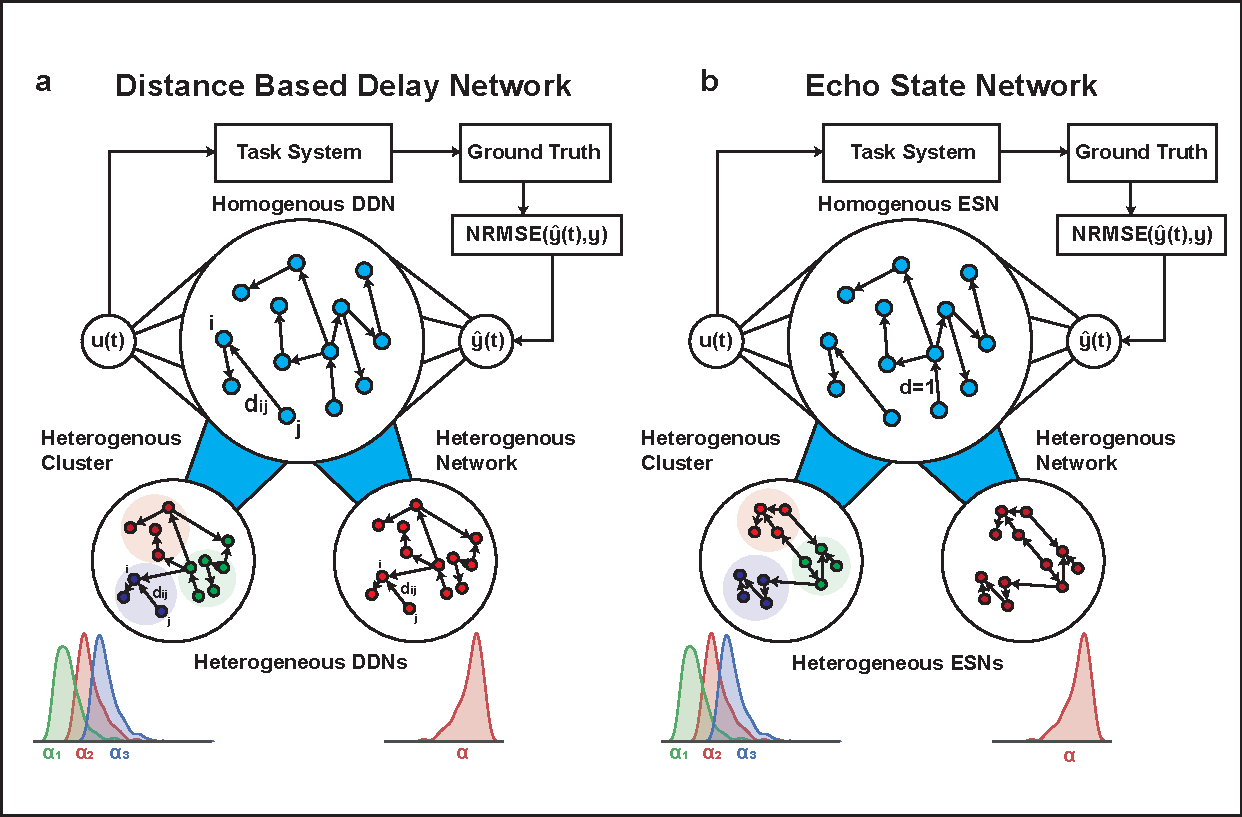
\includegraphics[width=\linewidth]{Figures/Ch_4/network_architecture.pdf}
    \caption{\textbf{Reservoir architecture and heterogeneity design in DDNs and ESNs:} \textbf{(a)} DDNs were made heterogeneous by introducing heterogeniety in delays ($\alpha$), cluster heterogeneity is designed by sampling delays from different distributions for each cluster, similarly, network heterogeneity is designed by sampling delays from a single distribution. \textbf{(b)} same heterogeneity designed for ESNs. It can also be seen that the key difference between ESNs and DDNs are the introduction of delays between units in case of DDNs.   }
    \label{fig:reservoir-arch}
\end{figure}
\subsection{Task Performance }
\subsubsection{NARMA 30}

In order to study the effect of heterogeneity in leak parameters in ESNs and DDNs, we evaluated the networks using their validation scores for each generation of CMA-ES algorithm shown in \textbf{Fig. \ref{fig:eval}a} while these networks learn to perform NARMA-30 task (see Methods). It can be seen that as the networks are optimized over generations, the validation scores lower for both ESNs and DDNs, but the NRMSE scores for DDNs, especially DDNs with network wide fixed decay, per cluster distributed decay and per cluster fixed decay are much lower than ESNs. It can also be seen that all ESNs are optimized to similar NRMSE scores. Interestingly, it can be seen that DDNs with per-cluster fixed decay out perform, DDNs with higher levels of heterogeneity, while the DDNs with network wide distributed decay showed similar performance as the ESNs. We also evaluated the performance of the best optimized networks on a test set shown in \textbf{Fig. \ref{fig:eval}b}, it can be seen that DDNs with network wide fixed decay has lower NRMSE score than ESNs. For per-cluster case, the performance of DDNs and ESNs are indistinguishable. 

\subsubsection{Mackey-Glass}
Similar to the NARMA-30 task we optimized ESNs and DDNs with varying levels of heterogeneity for Mackey-Glass time series prediction task (see Methods section ), we evaluated the performance of the networks using prediction horizon metric (see Methods section ), it can be seen from \textbf{Fig. \ref{fig:eval}b} that prediction horizons for validation run over generation of CMA-ES optimization for DDNs are consistently higher than the ESNs. It can also be seen that DDNs with network wide distributed decay performs the best among all the DDNs, reaching the prediction horizon of 500 steps. It is also noticeable that ESNs with per cluster distributed decay and network wide fixed decay perform the worse compared to all other variants. ESNs with network wide distributed decay and per cluster fixed decay perform objectively better, reaching a prediction horizon value of 300 steps.  Similar to the NARMA-30 taks, we evaluated the performance of the best optimized networks on a test set shown in \textbf{Fig. \ref{fig:eval}b}, it can be seen that DDNs with network wide fixed decay has lower NRMSE score than ESNs.

\begin{figure}
    \centering
    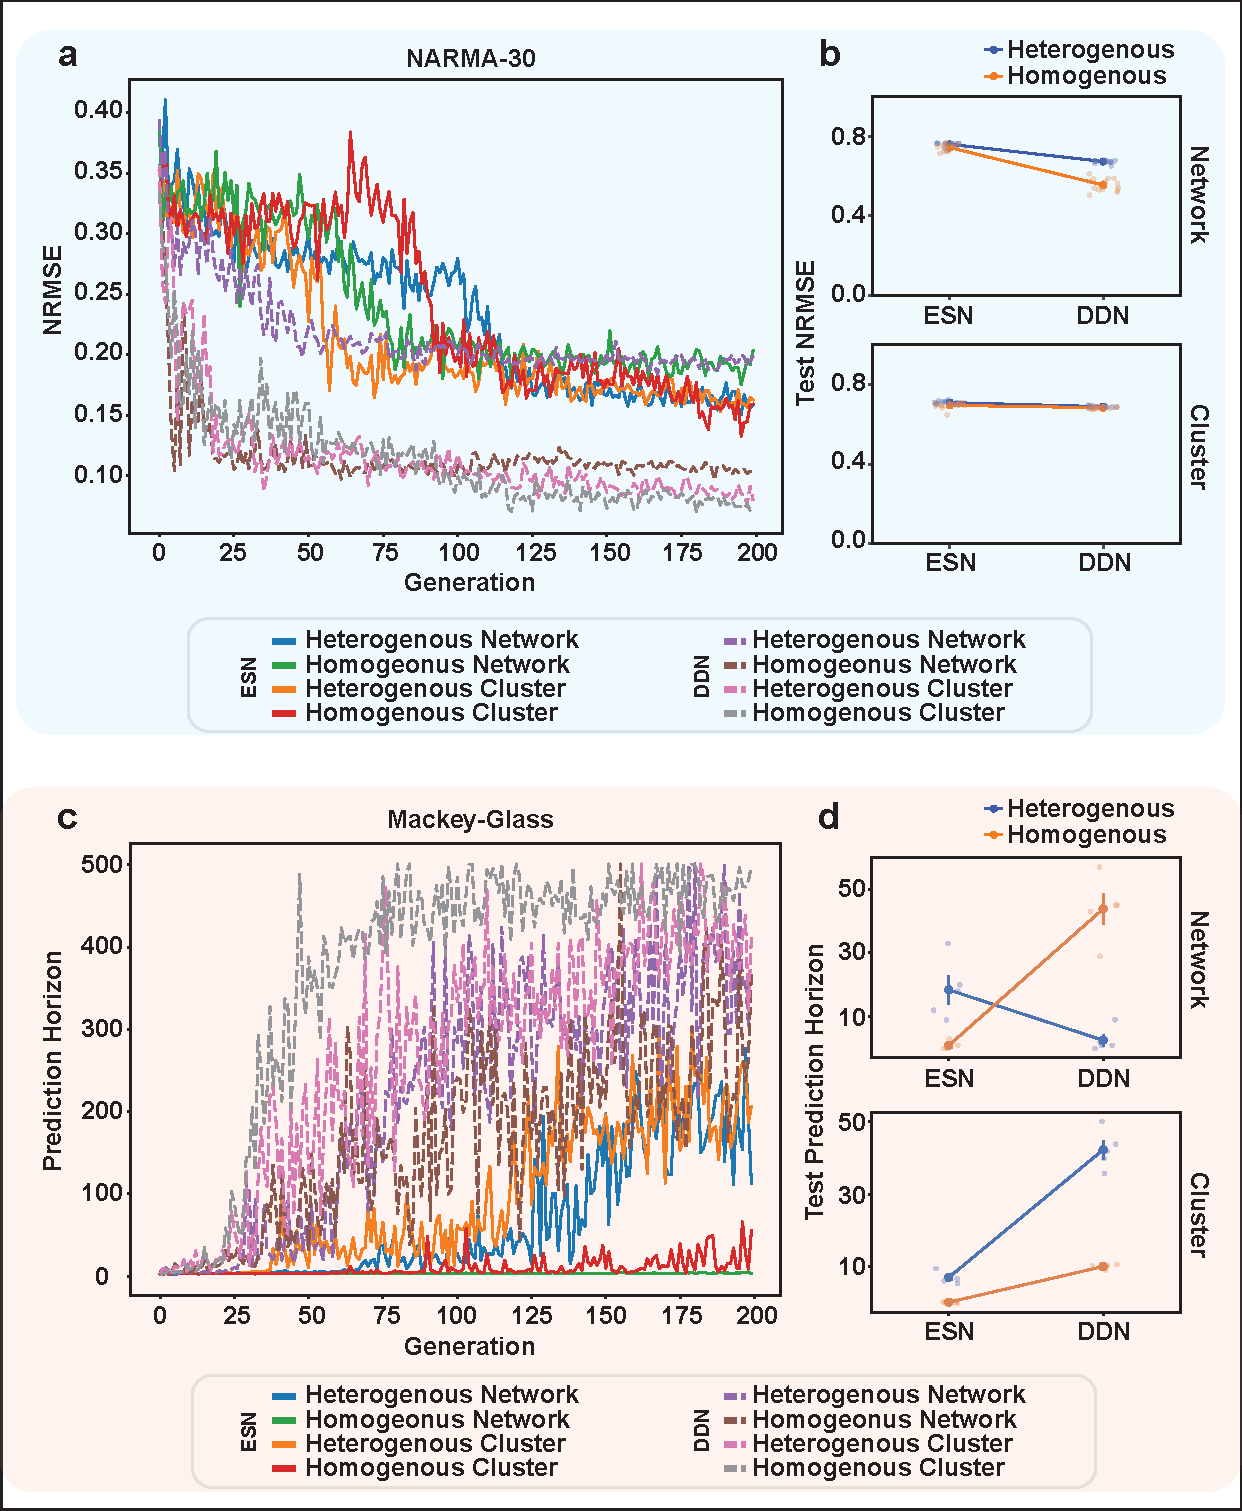
\includegraphics[width=\linewidth]{Figures/Ch_4/Task_performance.pdf}
    \caption{\textbf{Network performance for DDNs and ESNs with or without heterogeneity}: \textbf{(a)} Line plot shows the perforamce in terms of NRMSE over generation during CMA-ES optimization for DDNs and ESNs during NARMA 30 task.  
    }
    \label{fig:eval}
\end{figure}

\begin{figure}

\textbf{(b)} Test NRMSE for different network configurations for both ESNs and DDNs. It can be seen that DDNs with/without heterogeneity perform better than ESNs. \textbf{(c)} Performance of ESNs and DDNs with or without heterogeneity optimized for Mackey-Glass prediction task over generations of CMA-ES optimization. \textbf{(d)} Test performance of ESNs and DDNs optimized for Mackey-Glass timeseries prediction task, separated based on heterogeneity types.
\end{figure}

\subsection{Stability and Dimensionality}
\subsubsection{Maximum Lyapunov exponents}
In order to evaluate the advantage of intrinsic heterogeneity on ESNs and DDNs we calculated the largest lyapunov exponents of the sampled best networks while they perform the task (see Methods section). This was done in order to examine the stability of the network dynamics while the networks perform the task, we hypothesized that intrinsic decay heterogeneity might cause the networks to be more chaotic than their homogeneous counterparts. We evaluated the Maximum Lyapunov exponents for each network and heterogeneity types for different perturbation magnitudes ranging from $1e^{-1}$ to $1e^{-9}$. We perform this analysis for NARMA-30 and Mackey-Glass tasks separately, the results are summarized in \textbf{Fig. \ref{fig:lyapunov}a-b}. 

For NARMA-30 task (\textbf{Fig. \ref{fig:lyapunov}a}), it can be seen that for each perturbation magnitude, the largest lyapunov exponent are negative for all ESNs variants and are lower than DDNs, suggesting that ESNs have more contracting dynamic than DDNs despite the heterogeneity. The outlier to this observation is the ESN with network wide fixed delay, for which the lyapunov exponent is negative but invariant to the perturbation magnitude and comparable to DDNs. It is also important to observe that for all perturbation magnitudes, the highest perturbation yields the lowest exponent. In case of DDNs, the per cluster fixed decay configuration the maximum lyapunov exponent was invariant to the perturbation magnitude. The MLE for DNNs with network wide distributed decay and per cluster distributed decay were comparable, on the other hand, DDNs with network wide fixed decay shows a positive MLE for highest magnitude perturbation ($1e^{-1}$) suggesting chaotic dynamics. 

For Mackey-Glass timeseries prediction task (\textbf{Fig. \ref{fig:lyapunov}b}), it can be seen that for each perturbation magnitude, the largest lyapunov exponent are negative for all ESNs variants and are lower than DDNs, suggesting that ESNs have more contracting dynamic than DDNs for this task as well, despite the heterogeneity. It is also important to observe that for all perturbation magnitudes, the highest perturbation yields the lowest exponent just as in case of NARMA-30. The ESNs with network wide distributed decay were found to have the highest MLE among ESNs and the ESNs with per cluster fixed decay were found to have the lowest MLE. In case of DDNs, the per cluster fixed decay configuration shows a positive exponent for the  magnitude of $1e^-9$ and $1e^-7$. The MLE for DNNs with all other variants had comparable negative MLE for all each perturbation magnitude suggesting a stable contracting dynamic. 

\subsubsection{Dimensionality}
In order to further evaluate the usefulness of intrinsic heterogeneity in terms of recruiting reservoir units for performing the task, we calculated the dimensionality of the network using the network states while the network is driven by the task input. We hypothesized that intrinsic decay heterogeneity might increase the dimensionality of the network, improving the task performance. We drove the network with NARMA-30 and Mackey-Glass input for 2000 steps, and used the network state after 300 steps of warm-up period. For NARMA-30 task, we observed low dimensionality for all networks, the highest for ESN with fixed decay per cluster (D=15) and lowest for DDNs with network wide fixed decay (D=8), distributed decay per cluster (D=8) and fixed decay per cluster (D=8). Similarly, for Mackey-glass time series prediction task, we observe low dimensionality for all networks except for ESNs with distributed decay per cluster (D=98). The network with lowest dimension was found to be DDNs with fixed decay per cluster. Overall, this shows that both ESNs and DDNs do not recruit a high number of units in order to perform both NARMA-30 and Mackey-glass tasks.      

\begin{figure}[!htpb]
    \centering
    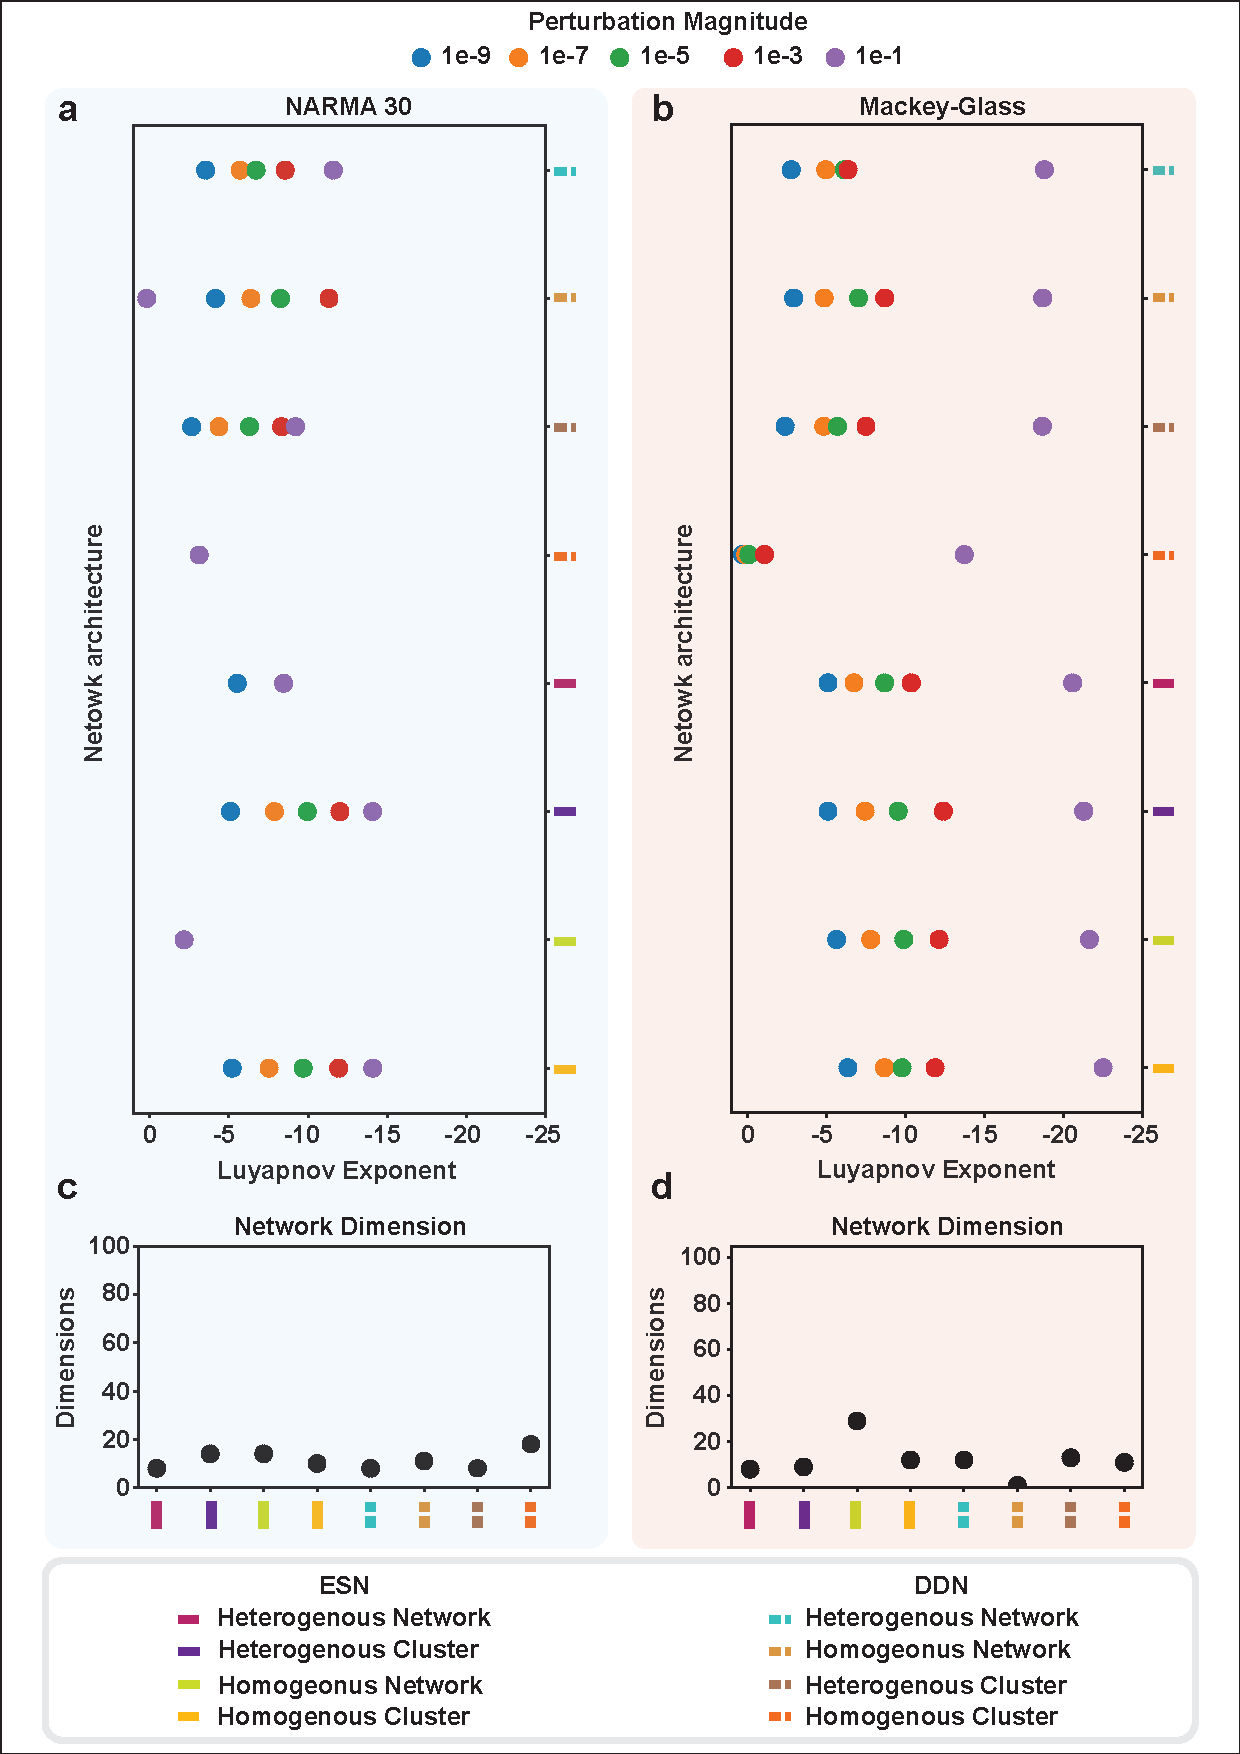
\includegraphics[width=0.8\linewidth]{Figures/Ch_4/Luyapnov_dimensions.pdf}
    \caption{\textbf{Dynamics based on Lyapunov exponent and dimensionality of optimized networks:} \textbf{(a-b)} shows the Lyapunov exponents of the optimized networks while performing the NARMA 30  (blue background) and Mackey-Glass (red background). \textbf{(c-d)} shows the network dimensionality while performing the NARMA 30 (blue background) and Mackey-Glass timeseries prediction tasks (red background).}
    \label{fig:lyapunov}
\end{figure}

\subsection{Linear Memory capacity}

In order to understand if intrinsic decay heterogeneity has an effect on the memory of ESNs and DDNs, especially to see if networks with heterogeneous decay parameters change the way networks store temporal information, especially the number of time steps these networks can recall information from, we calculated the linear memory capacity (see methods section). We used the maximum delay of 40 steps. The observed linear memory capacity for each network variant is summarized on \textbf{Fig. \ref{fig:MC}}. 


For the NARMA-30 task (\textbf{Fig. \ref{fig:MC} left}), it can be seen that every ESN variant has the capacity to recall from upto 20 time steps ago and the capacity is distributed over all the steps between 0 and 20, we do not observe a stark improvement in the memory capacity as a result of heterogeneity.  On the other hand, DDNs show a much more nuanced difference in terms of memory distribution for NARMA-30 task, DDNs with fixed decay per cluster show a concentration of capacity at 3 different time steps, while DDNs with distributed decay per cluster show a prominent concentration at two delay steps. It is also clearly observed that DDNs do not utilize the time window closer to the input, creating a except for DDNs with network wide fixed decay. This suggests that ESNs have limited mobility to recall the past steps in order to perfrom the task, and decay heterogeneity doesn't provide any improvement on this. While, DDNs scatter the capacity more sparsely, thus utilizing the past states more strategically.         

For the Mackey-Glass time series prediction task (\textbf{Fig. \ref{fig:MC} left}), it can be seen that every ESN variant ustilizes just a few past states from when the input is received, most of the capacity is recruited from just the previous step, we do not observe a stark improvement in the memory capacity as a result of heterogeneity for the case of Mackey-Glass as well. On the other hand, DDNs show a much more variability, DDNs with network wide distributed decay and DDNs with distributed decay per cluster, show a wide spread capacity over multiple delay steps, while DDNs with fixed values show a concentration of capacity around 10 time steps ago. 

This goes to show that while for ESNs, the decay heterogeneity doesn't change drastically, for DDNs, the memory capacity is altered due to decay heterogeneity, therefore aiding in task performance. 


\begin{figure}
    \centering
    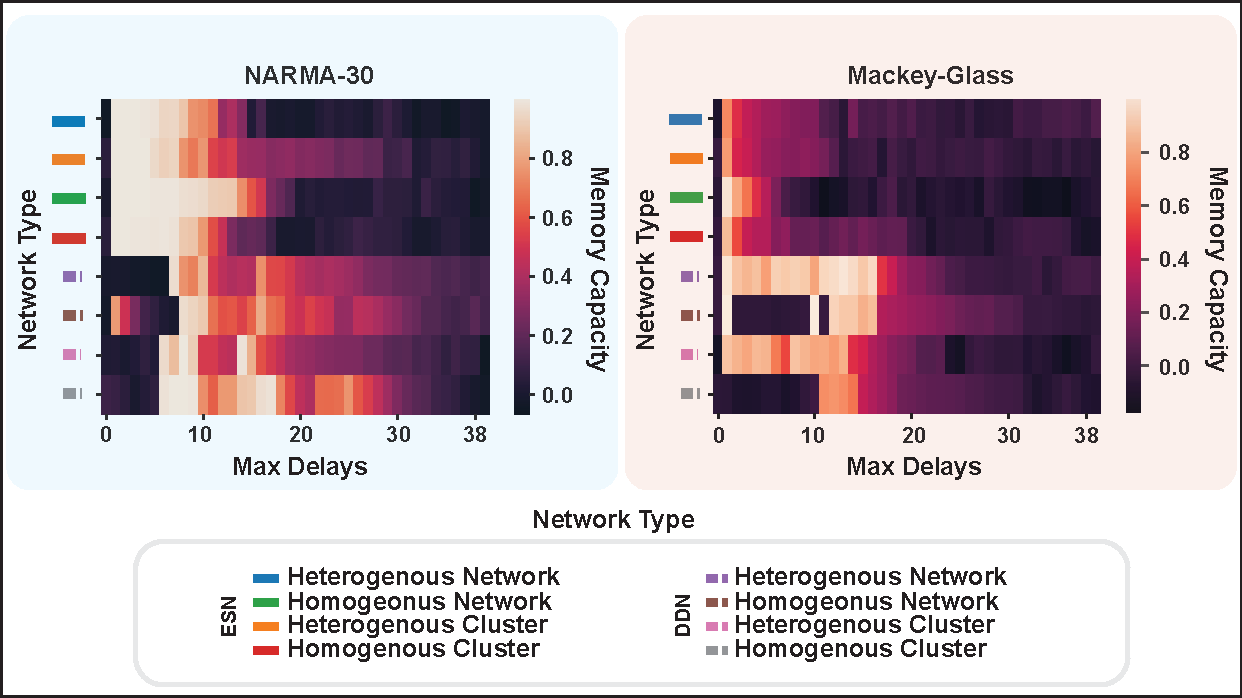
\includegraphics[width=\linewidth]{Figures/Ch_4/LInear MC.pdf}
    \caption{\textbf{Linear Memory Capacity of optimized networks}: \textbf{(Left)} Linear memory capacity of the networks optimized for NARMA 30 task for different delays. \textbf{(Right)} Linear memory capacity of the networks optimized for Mackey-Glass time series prediction task for different delays. }
    \label{fig:MC}
\end{figure}


\newpage

\newpage
\section{Discussion}


This study aimed at studying the effect of timescale (decay parameter) heterogeneity of individual units in reservoir networks on their computational performance, particularly in ESNs and DDNs. Set across two benchmark tasks namely, NARMA-30 and Mackey-Glass, and across four heterogeneity configurations. We found that across all heterogeneity configurations, DDNs outperform ESNs in both tasks. This confirms previous work showing that delay-based architectures are better suited for memory-intensive tasks \cite{iacob2022distance}, this can be because the introduction of time delays enables more flexible temporal dynamics, even more so than inherent decay, rendering inherent decay redundant. We observed that ESNs trained on NARMA-30 task, homogeneous cluster performs the best. But not for the Mackey-Glass task, where ESNs with Heterogeneous cluster, shows the best performance. Surprisingly, homogeneous network DDNs outperform heterogeneous network ESNs, suggesting that architectural delay mechanisms alone offer substantial computational benefits extending the hypothesis \cite{tanaka2022reservoir} that diverse timescales enhance network performance in both DDNs and ESNs.

The ultimate best-performing configuration across both tasks was the homogeneous cluster DDNs. This suggests that structured, modular heterogeneity in decay parameters is more beneficial than randomly distributed heterogeneity. One likely reason is that this setup creates functionally specialized subpopulations with different integration windows, which quite common in biological neural circuits. It allows the reservoir to simultaneously retain short and long term dependencies spread across multiple units. These results support the hypothesis rooted in neuroscience that the diversity of timescales is functionally beneficial for temporal processing and memory \cite{Lundqvist2016gamma, Runyan2017timescales, Cavanagh2020diverse}. 

Contrary to our initial hypothesis, networks with decay heterogeneity did not show increased instability. In fact, all ESNs remained in a contracting regime, with strongly negative Lyapunov exponents across perturbation magnitudes. DDNs were more variable, with some configurations (e.g., Homogeneous network) approaching neutral or even slightly positive exponents under high perturbation. This suggests that DDNs trade off stability for richer dynamics, and that heterogeneity does not necessarily lead to chaotic or unstable behavior. Interestingly, for all network types, the largest perturbation magnitude yielded the most negative Lyapunov exponent. This is likely due to saturation or nonlinear contraction in state space, and highlights the importance of evaluating stability in the local (infinitesimal) regime to interpret true Lyapunov behavior.

We hypothesized that decay heterogeneity would increase the effective dimensionality of the network enabling richer representations. This was not supported. Most networks exhibited relatively low-dimensional dynamics, with little difference between configurations. This could mean that the tasks at hand do not require high-dimensional embeddings, or that the reservoirs learn to compress relevant dynamics efficiently regardless of heterogeneity. It may also suggest that stability and memory, not dimensionality, are the primary contributors to performance in this setting.

Linear memory capacity analysis revealed a more nuanced story. While ESNs showed limited changes across heterogeneity types, DDNs exhibited significant differences in how memory was distributed. Notably, DDNs with distributed decay showed wider memory spread, while fixed-decay variants concentrated memory at specific lags. This suggests that decay heterogeneity allows DDNs to strategically allocate memory a critical property for tasks like NARMA, where both recent and delayed inputs matter. This behavior was absent in ESNs, which tended to have more rigid, shallow memory profiles regardless of heterogeneity.

This study is limited to two benchmark tasks and a specific class of recurrent models. Future work should explore: Broader tasks, including those involving categorical sequence prediction or noisy real-world data, other forms of heterogeneity (e.g., in connectivity, input weights), how decay heterogeneity interacts with delay heterogeneity under more complex learning rules or online adaptation. It would also be valuable to explore the Information processing capacity of these systems, and how dimensionality evolves over time or under different input statistics.

Our results suggest that introducing modular heterogeneity in decay dynamics can meaningfully improve performance and memory organization in reservoir networks particularly when paired with architectural delays. From a neuroscience perspective, this supports the idea that diverse time constants in biological systems are not incidental, but serve computational roles such as memory stratification and temporal coding.

From an engineering viewpoint, these findings argue for designing non-uniform, structured reservoirs in artificial systems, especially for tasks involving long-range dependencies or multi-timescale dynamics. Rather than tuning a single decay or leak parameter, practitioners could benefit from multi-cluster architectures with targeted decay profiles.


\newpage


\begin{spacing}{1.0} % Set the line spacing to single spacing
\fontsize{8pt}{8pt}\selectfont
\bibliographystyle{apalike} %%%%Changed
\renewcommand{\bibname}{References}
\bibliography{All_bibtex} %%%%Changed
\end{spacing} % restore the line spacing to original
% \printbibliography